

% \begin{center}
% 	{\scriptsize
% 		\begin{tabularx}{\textwidth}{p{0.2\textwidth}|p{0.6\textwidth}|p{0.1\textwidth}}
% 			\caption{Summary of methods for reaching the objectives} \label{tab:methods_per_objective} \\
% 			\hline 
% 			\hline 
% 			\textbf{Objectives} & 
% 			\textbf{Methods} &
% 			\textbf{Locations}\\ 
% 			\hline 
% 			\endfirsthead
% 			\multicolumn{3}{c}%
% 			{\textit{Continued from previous page}} \\
% 			\hline
% 			\hline 
% 			\textbf{Objectives} & 
% 			\textbf{Methods} &
% 			\textbf{Locations}\\ 
% 			\hline 
% 			\endhead
% 			\hline 
% 			\multicolumn{3}{r}{\textit{Continued on next page}} \\ 
% 			\endfoot
% 			\hline 
% 			\endlastfoot
% 			\hline
			
			
% 			\Paste{GO} & \blindlist{enumerate} & Sec.~\ref{sec:implement} on p.~\pageref{sec:implement}\\ \hline
			
			
% 			\Paste{SO1} & \blindlist{enumerate} & Sec.~\ref{sec:implement} on p.~\pageref{sec:implement} \\ \hline
			
			
% 			\Paste{SO2} & \blindlist{enumerate} & Sec.~\ref{sec:implement} on p.~\pageref{sec:implement}\\ \hline
			
			
% 			\Paste{SO3} & \blindlist{enumerate} & Sec.~\ref{sec:implement} on p.~\pageref{sec:implement}\\ \hline
			
			
% 			\Paste{SO4} & \blindlist{enumerate} & Sec.~\ref{sec:implement} on p.~\pageref{sec:implement} \\ \hline
			
			
% 			\Paste{SO5} & \blindlist{enumerate} & Sec.~\ref{sec:implement} on p.~\pageref{sec:implement} \\ \hline
			
% 		\end{tabularx}
% 	}
% \end{center}


\section{Methodology}
\begin{figure}
	\centering
	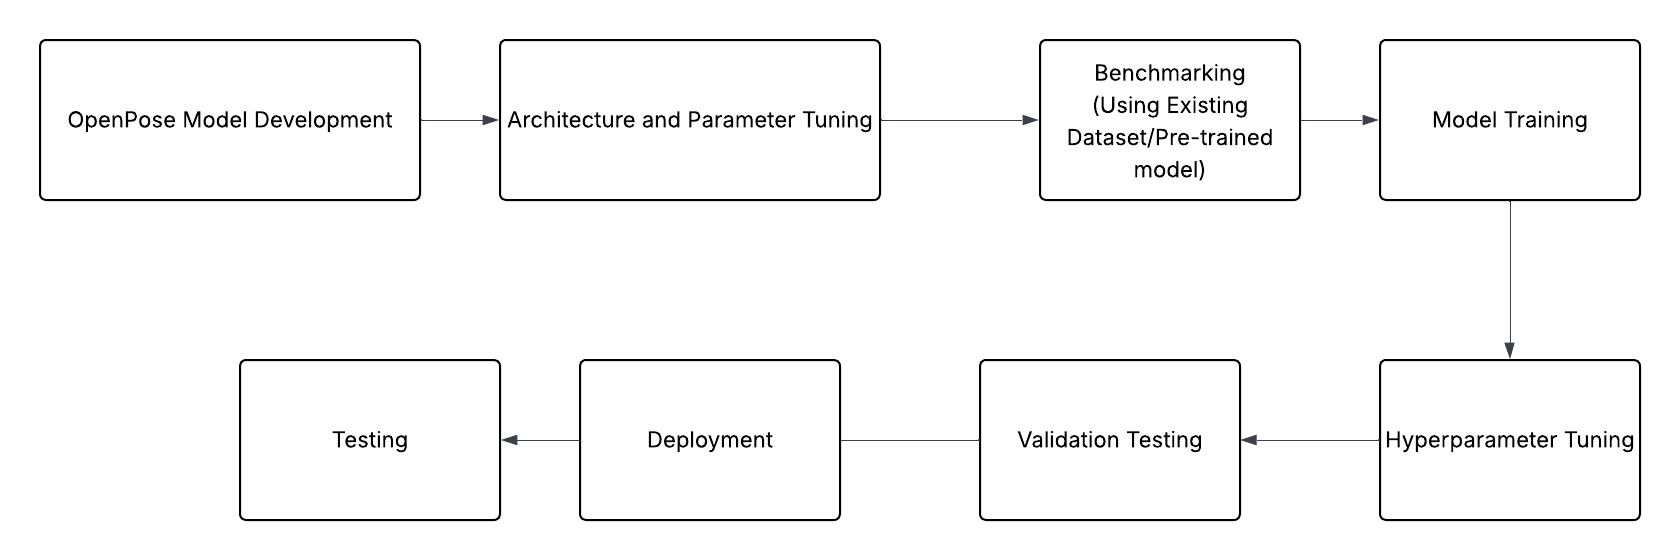
\includegraphics[width=0.8\textwidth]{methodology.png}
	\caption{Methodology Flowchart}
	\label{fig:methodology_flowchart}
\end{figure}

\AtBeginEnvironment{longtable}{\tiny}
\begin{longtable}{|p{2.5cm}|p{2.5cm}|p{2.5cm}|p{2.5cm}|}
\caption{Methods for Achieving Specific Objectives for Tinikling Detector} \label{tab:tinikling_methods} \\

\hline
\textbf{Specific Objective (SO)} & \textbf{Focus} & \textbf{Methodology} & \textbf{Expected Outcome} \\ \hline
\endfirsthead

\multicolumn{4}{c}{{\bfseries Table \thetable\ (continued)}} \\ \hline
\textbf{Specific Objective (SO)} & \textbf{Focus} & \textbf{Methodology} & \textbf{Expected Outcome} \\ \hline
\endhead

\hline \multicolumn{4}{r}{{Continued on next page}} \\ \hline
\endfoot

\hline
\endlastfoot

\textbf{SO1} & To develop a real-time pose estimation pipeline for Tinikling & Use MediaPipe's hand and pose estimation to track key skeletal landmarks in real time from webcam input. Process the frames at 30 fps or higher & Pose landmarks detected with at least 90\% accuracy and 30 fps. Reliable identification of Tinikling steps from skeletal data. \\ \hline

\textbf{SO2} & To make the pose estimation model robust to lighting, background clutter, and user variation & Use data augmentation (e.g., lighting, background noise, angles) and landmark-based representations to improve model robustness & Enhanced robustness under varying conditions with a minimum pose detection accuracy of 85\% across diverse backgrounds. \\ \hline

\textbf{SO3} & To design a scoring and feedback system for Tinikling steps & Integrate a scoring system that compares detected poses with reference choreography using temporal alignment methods like Dynamic Time Warping (DTW) & Real-time feedback with numerical scores (0–100) for step-by-step accuracy breakdowns within 1 second after performance. \\ \hline

\textbf{SO4} & To develop a desktop-based user interface with real-time feedback & Implement an intuitive user interface that provides visual and audio feedback, integrating with the pose estimation pipeline for immediate performance assessment & Real-time visual and audio cues within 200 ms, with performance scores displayed after each session. \\ \hline

\textbf{SO5} & To evaluate system performance and usability through testing & Conduct controlled testing with at least 10 participants, measuring accuracy, latency, and user satisfaction using surveys and performance metrics & Performance evaluation with \(\geq 80\%\) positive feedback and refined system based on accuracy and latency benchmarks. \\ \hline

\end{longtable}

\section{Design Considerations}

\subsection{Sensor choice, representation, and robustness}
A study by Tölgyessy, Dekan, and Chovanec (2021) demonstrated that Kinect-family depth sensors produce explicit 3D skeletons and give higher joint fidelity in controlled settings, but the accuracy falls with occlusion, off-axis views, and increased distance. Zhang et al. (2020) described MediaPipe, which yields compact 2D/3D landmark coordinates from ordinary RGB cameras and runs in real time on mobile devices. Therefore, designers often choose landmarks for rapid, lightweight prototypes and mobile deployment, and reserve depth or IR systems for installation-grade fidelity when hardware is available. To reduce real-world failure modes, practitioners apply photometric and background augmentation and synthetic occlusions during training, and they add a short calibration step so system metrics align with an individual user’s range of motion.

\subsection{Temporal alignment and scoring}
Dance is a temporal activity and should be compared as a sequence rather than as isolated frames. Yu and Xiong (2019) demonstrate that Dynamic Time Warping (DTW) can align noisy, tempo-varying Kinect skeleton sequences and convert DTW distances into meaningful performance scores. Rallis et al. (2019) apply DTW to choreographic trajectories and show it can match patterns across high-precision (VICON) and low-cost (Kinect) capture systems. Thus, a practical scoring pipeline first aligns sequences with DTW (or a constrained variant) and then evaluates local spatial metrics such as joint-angle differences or normalized trajectory distances to produce interpretable, per-segment correctness scores.

\subsection{Real-time feedback, segmentation, and pedagogy}
Lin (2015) finds that immediate, clear feedback in dance exergames improves engagement and supports learning. Zhang et al. (2020) show that on-device landmark extraction can run at real-time rates suitable for low-latency feedback. Combining these results suggests a two-tier runtime design: use a fast, coarse matcher (enabled by on-device landmarks) for instant cues, and run a slower, higher-precision alignment and scoring pass for final grading. Breaking choreography into short labeled segments also simplifies alignment and reduces error accumulation; Rallis et al. (2019) illustrate that segment- or trajectory-level matching better supports choreographic retrieval and per-segment feedback.

\subsection{Accessibility, personalization, and evaluation}
Yu and Xiong (2019) convert DTW distances into calibrated percentage scores, which supports per-user calibration and comparison against an individualized baseline. Tölgyessy et al. (2021) recommend measuring sensor-level metrics such as joint error and dropout rates when choosing a capture modality. Therefore, system designs should include adjustable sensitivity, alternate gesture mappings, and user profiles, and evaluation should combine sensor metrics (joint error, dropout, latency) with human-centered measures (perceived accuracy, engagement, and learning gain) to justify architecture and scoring choices.

\section{Theoretical Considerations}

\subsection{Human Pose Estimation}

Human pose estimation is the process of predicting the pose of human body parts. The data are typically stemming from RBD images or videos. Given that certain motions are motivated by human actions, detecting poses is a critical aspect of human action recognition (Song et al., 2021). It has a wide range of applications such as human-computer interaction, motion analysis, augmented reality, and virtual reality. The resulting output of human pose estimation is a skeleton-like representation of the human body consisting of nodes and limbs (Zheng et al, 2020)). There are 2 main types of human pose estimation, namely 2D and 3D. 2D pose estimation consists of predicting the posture of each of the body’s key points in a 2D plane, considering the X and Y axis. As for 3D pose estimation, it considers the Z axis, situating each point in a 3D space. It goes without saying that the 3D estimation would be much more difficult in comparison to 2D estimation in process or complexity due to underlying issues which may manifest such as noisy backgrounds, clothing, lighting, undetected joints, or occlusion (Ben Gamra \& Akhloufi, 2021).  


\subsection{Human Action Recognition}

	Human action recognition, otherwise known as HAR. is the process of detecting human actions in order to classify them through single sensor data, RBD image or video data, or three-dimensional depth and inertial data (Sakar et al., 2022). In the field of computer vision, one of the most challenging aspects of it is the automatic and precise identification of human activity. Over the years, there has been a significant increase in feature learning-based representations for human action recognition as a result of the widespread utilization of deep learning-based features. There are various applications of Human action recognition. For instance, automated surveillance systems make use of AI and machine learning algorithms in order to identify human actions for the sake of safety and security. Such a task, however, is made difficult due to various factors such as changing online environments, occlusion, different viewpoints, execution pace and biometric change. Not only this, but the human body also varies from person to person in factors such as size, appearances, and shapes. However, advancements in Convolutional Neural Networks, otherwise known as CNNs, resulted in significant progress for human action recognition through improvements on classification, segmentation and object detection. This largely applies more on image-related tasks  rather than videos as neural network models struggle to capture temporal information in videos due to a lack of substantial datasets (Morshed et al., 2022). 


\section{Summary}
In this chapter, we discussed the methodology and design considerations for building a real-time Tinikling learning application using human pose estimation. The main focus is on developing a pose estimation pipeline, using MediaPipe for landmark detection, and integrating a scoring system for feedback based on detected poses. Several methods are employed to ensure robustness against environmental challenges such as lighting and background clutter, and real-time feedback is provided to guide users in learning the Tinikling dance steps.

\gls{not:It}